\chapter{Opis struktury projektu}
\label{cha:struktura}

% ------------------------------------------------------------------------

\section{Struktura kodu projektu}

Projekt symulatora sklepu interentowego napisany został w języku obiektowym Java, zatem do jego uruchomienia niezbędne będzie oprogramwanie Java w wersji 11+. 
Projekt podzielony został na sześć pakietów:
\begin{itemize}
    \item	userPCG,
    \item	productPCG,
    \item	orderPCG,
    \item   shoppingCartPCG,
    \item   GUI,
    \item   figures,
    \item   database.
\end{itemize}

% ------------------------------------------------------------------------

\subsection{Użytkownicy}

Zarządanie użytkownikami, klasy i metody im poświęcone znajdują się w pakiecie \texttt{userPCG}. Klasa \texttt{User} zawiera pola informujące o danych użytkownika,
konstruktory oraz podstawowe metody, takie jak gettery i settery. Wewnątrz klasy \texttt{userServices} znajdują się kluczowe metody do zarządania użytkownikami w panelach klienta, jak i administratora, takie 
jak np. metoda do rejestrowania nowego użytkownika, przedstawiona na \listingname~\ref{registerUser}.

\lstinputlisting[caption= Metoda do rejestrowania nowych użytkowników, label=registerUser, style = javaStyle]{src/registerUser.java}

Natomiast zarządaniem aktualnie zalogowanym użytkownikiem zajmuje się klasa \texttt{UserSession}.
Każdy typ użytkownika ma przypisaną rolę, której odpowiada warość liczbowa, co zaprezentowane jest w \tablename~\ref{tabRole}.

\begin{table}[H]
    \caption{Role użytkowników}
    \label{tabRole}
    \centering
    \begin{tabular}{ccc}
        \toprule
        \textbf{rola} & \textbf{wartość liczbowa} \\ \toprule
        klient           & 1                              \\
        administrator           & 2                               \\
        gość           & 3                              \\
    \bottomrule
    \end{tabular}
\end{table}

Poszczególne typy użytkowników mają dostęp do różnych działań w aplikacji.

% ------------------------------------------------------------------------

\subsection{Produkty}

Wszystkie potrzebne informacje i metody do zarządzania produktami w sklepie zawarte są w pakiecie \texttt{productPCG}.
Każdy typ sprzedawanego produktu, czyli książki fizyczne, ebooki i audiobooki posiadają własne klasy (\texttt{PhysicalBook}, \texttt{Ebook}, \texttt{Audiobook}), które dziedziczą
po klasie abstrakcyjnej \texttt{Book}, która to z kolei implementuje interfejs \texttt{Product}, co przedstawia \figurename~\ref{fig2}. Diagram został sporządzony na stronie: \url{https://www.drawio.com/}.

\begin{figure}[H]
    \centering
    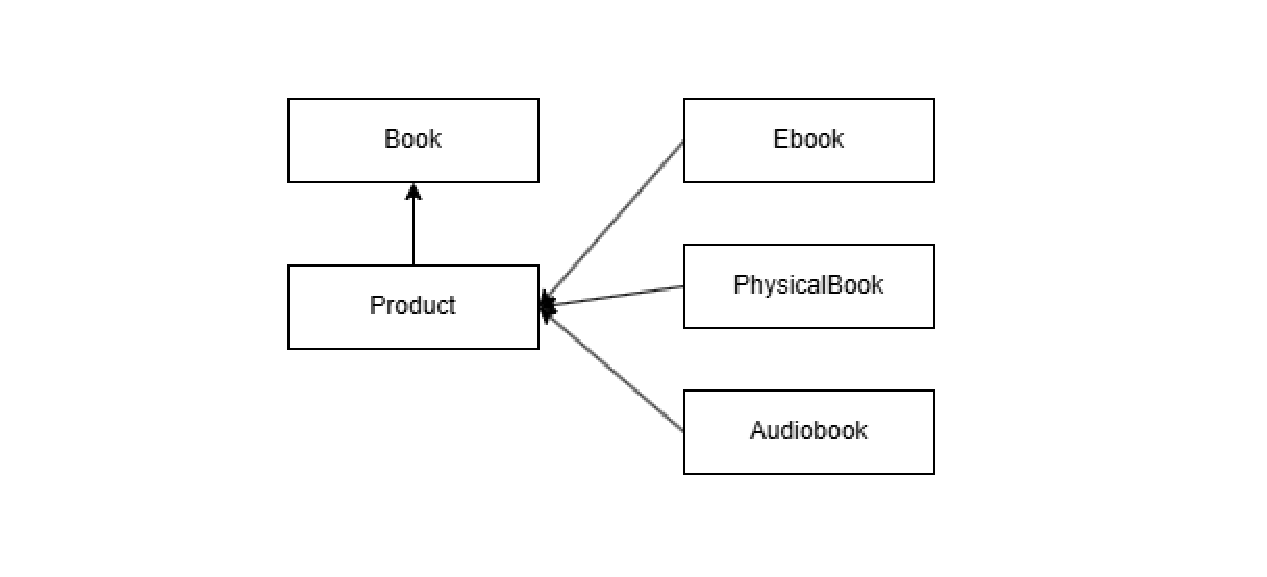
\includegraphics[width=\linewidth]{figures/fig_0002.eps}\\
    \caption{Diagram dziedziczenia klas produktów.\label{fig2}}
\end{figure}

Pakiet zawiera również enum \texttt{BookCategory}, w którym przechowywane są kategorie sprzedawanych książek. 
Enum przedstawiono na \listingname~\ref{enum}.
\lstinputlisting[caption= Enum kategorii książek, label=enum, style = javaStyle]{src/enum.java}

Kluczowe metody do zarządzania produktami znajdują się w klasie \texttt{ProductServices}.
Zawiera między innymi metody do dodawania, usuwania, pobierania, a także metody aktualizowania danych podstawowych produktu (\texttt{Book}) oraz pochodne 
metody do aktualizowania danych specyficznych dla konkretnych typów produktów (\texttt{PhysicalBook}, \texttt{Ebook}, \texttt{Audiobook}), których przykłady 
podano w \listingname~\ref{updateBook} i \listingname~\ref{updateEbook}.
\lstinputlisting[caption= Metoda aktualizująca podstawowe dane produktu, label=updateBook, style = javaStyle]{src/updateBook.java}
\lstinputlisting[caption= Metoda aktualizująca specyficzne dane dla Ebooka, label=updateEbook, style = javaStyle]{src/updateEbook.java}

Rozbudowany unikalny identyfikator produktu jest generowany automatycznie dzięki użyciu metody \texttt{randomUUID()} ze standardowej klasy \texttt{UUID}.

Wewnątrz klasy \texttt{ProductServices} umieszona została dodatkowo klasa wewnętrzna \texttt{ProductInfo}, która zawiera konkretne pola ułatwiające przechowywanie
informacji o produktach, np. w katalogach i koszyku. Zaprezentowana została ona w \listingname~\ref{productInfo}.
\lstinputlisting[caption= Wewnętrzna klasa ProductInfo, label=productInfo, style = javaStyle]{src/ProductInfo.java}

% ------------------------------------------------------------------------

\subsection{Koszyk i Zamówienia}

Obsługa zamówień odbywa się przy pomocy klasy \texttt{OrderServices} w pakiecie \texttt{orderPCG}. Oprócz metody do tworzenia nowego zamówienia i aktualizacji statusu zamówienia, dostępne są również metody 
tworzące listy wszystkich zamówień wykorzystujące wewnętrzne klasy \texttt{OrderInfo}, z polami dotyczącymi danych samego zamówinienia, a także \texttt{OrderItemInfo}, z polami produktów w zamówieniu.

Koszyk z produktami działający przy pomocy klasy \texttt{ShoppingCart} zawiera listę produktów, która później trafia do zamówienia, a także metody do dodawania dodawania i usuwania produktów z niego.

% ------------------------------------------------------------------------

\subsection{Materiały}

Jedynym zewnętrznym materiałem wykorzystywanym w aplikacji jest \texttt{book.png}, przechowywany w \texttt{figures}, materiał ten służy jako logo, wyświetlane w banerze na każdej stronie sklepu.
Logo to, przedstawione na  \figurename~\ref{fig3}, pobrane zostało z \url{https://icons8.com/icons/set/book}.
\begin{figure}[H]
    \centering
    
\includegraphics[width=\linewidth]{figures/fig_0003.eps}\\
    \caption{obrazek książki wykorzystany w aplikacji.\label{fig3}}
\end{figure}

% ------------------------------------------------------------------------

\section{Baza danych}

% ------------------------------------------------------------------------

W symulatorze sklepu internetowego, dane przechowywane i zarządzane są za pomocą relacyjnej bazy danych MySQL.

\subsection{Połączenie z bazą danych}

Połączenie z bazą danych odbywa się za pomocą interfejsu API, JDBC. Baza danych testowo przechowywana jest na serwerze pakietu XAMPP, natomiast połącznie z serwerem przeprowadzone zostało poprzez
implementację do projektu \texttt{Connector/J}, dostępnego na \url{https://dev.mysql.com/downloads/connector/j/}.

Celem łatwego łączenia się z bazą danych utworzona została klasa \texttt{DBConnection}, przedstawiona w \listingname~\ref{database}.
\lstinputlisting[caption= Klasa łączenia się z bazą danych, label=database, style = javaStyle]{src/database.java}

% ------------------------------------------------------------------------

\subsection{Struktura bazy danych}

Struktura bazy, zaprojektowana została w taki sposób, aby umożliwić łatwe zarządzanie informacjami o użytkownikach, produktach oraz zamówieniach.
Baza danych składa się z tabel głównych \texttt{users}, \texttt{products} i \texttt{orders}, a także tabel \texttt{physical book}, \texttt{ebooks}, \texttt{audiobooks} z danymi specyficznymi dla 
konkretnych typów książek, tabeli \texttt{order items}, zawierającej dane o produktach z zamówień oraz tabel pomocniczych \texttt{categories} i \texttt{roles}. Diagram ERD przedstawiono na \figurename~\ref{fig4}.

\begin{figure}[H]
    \centering
    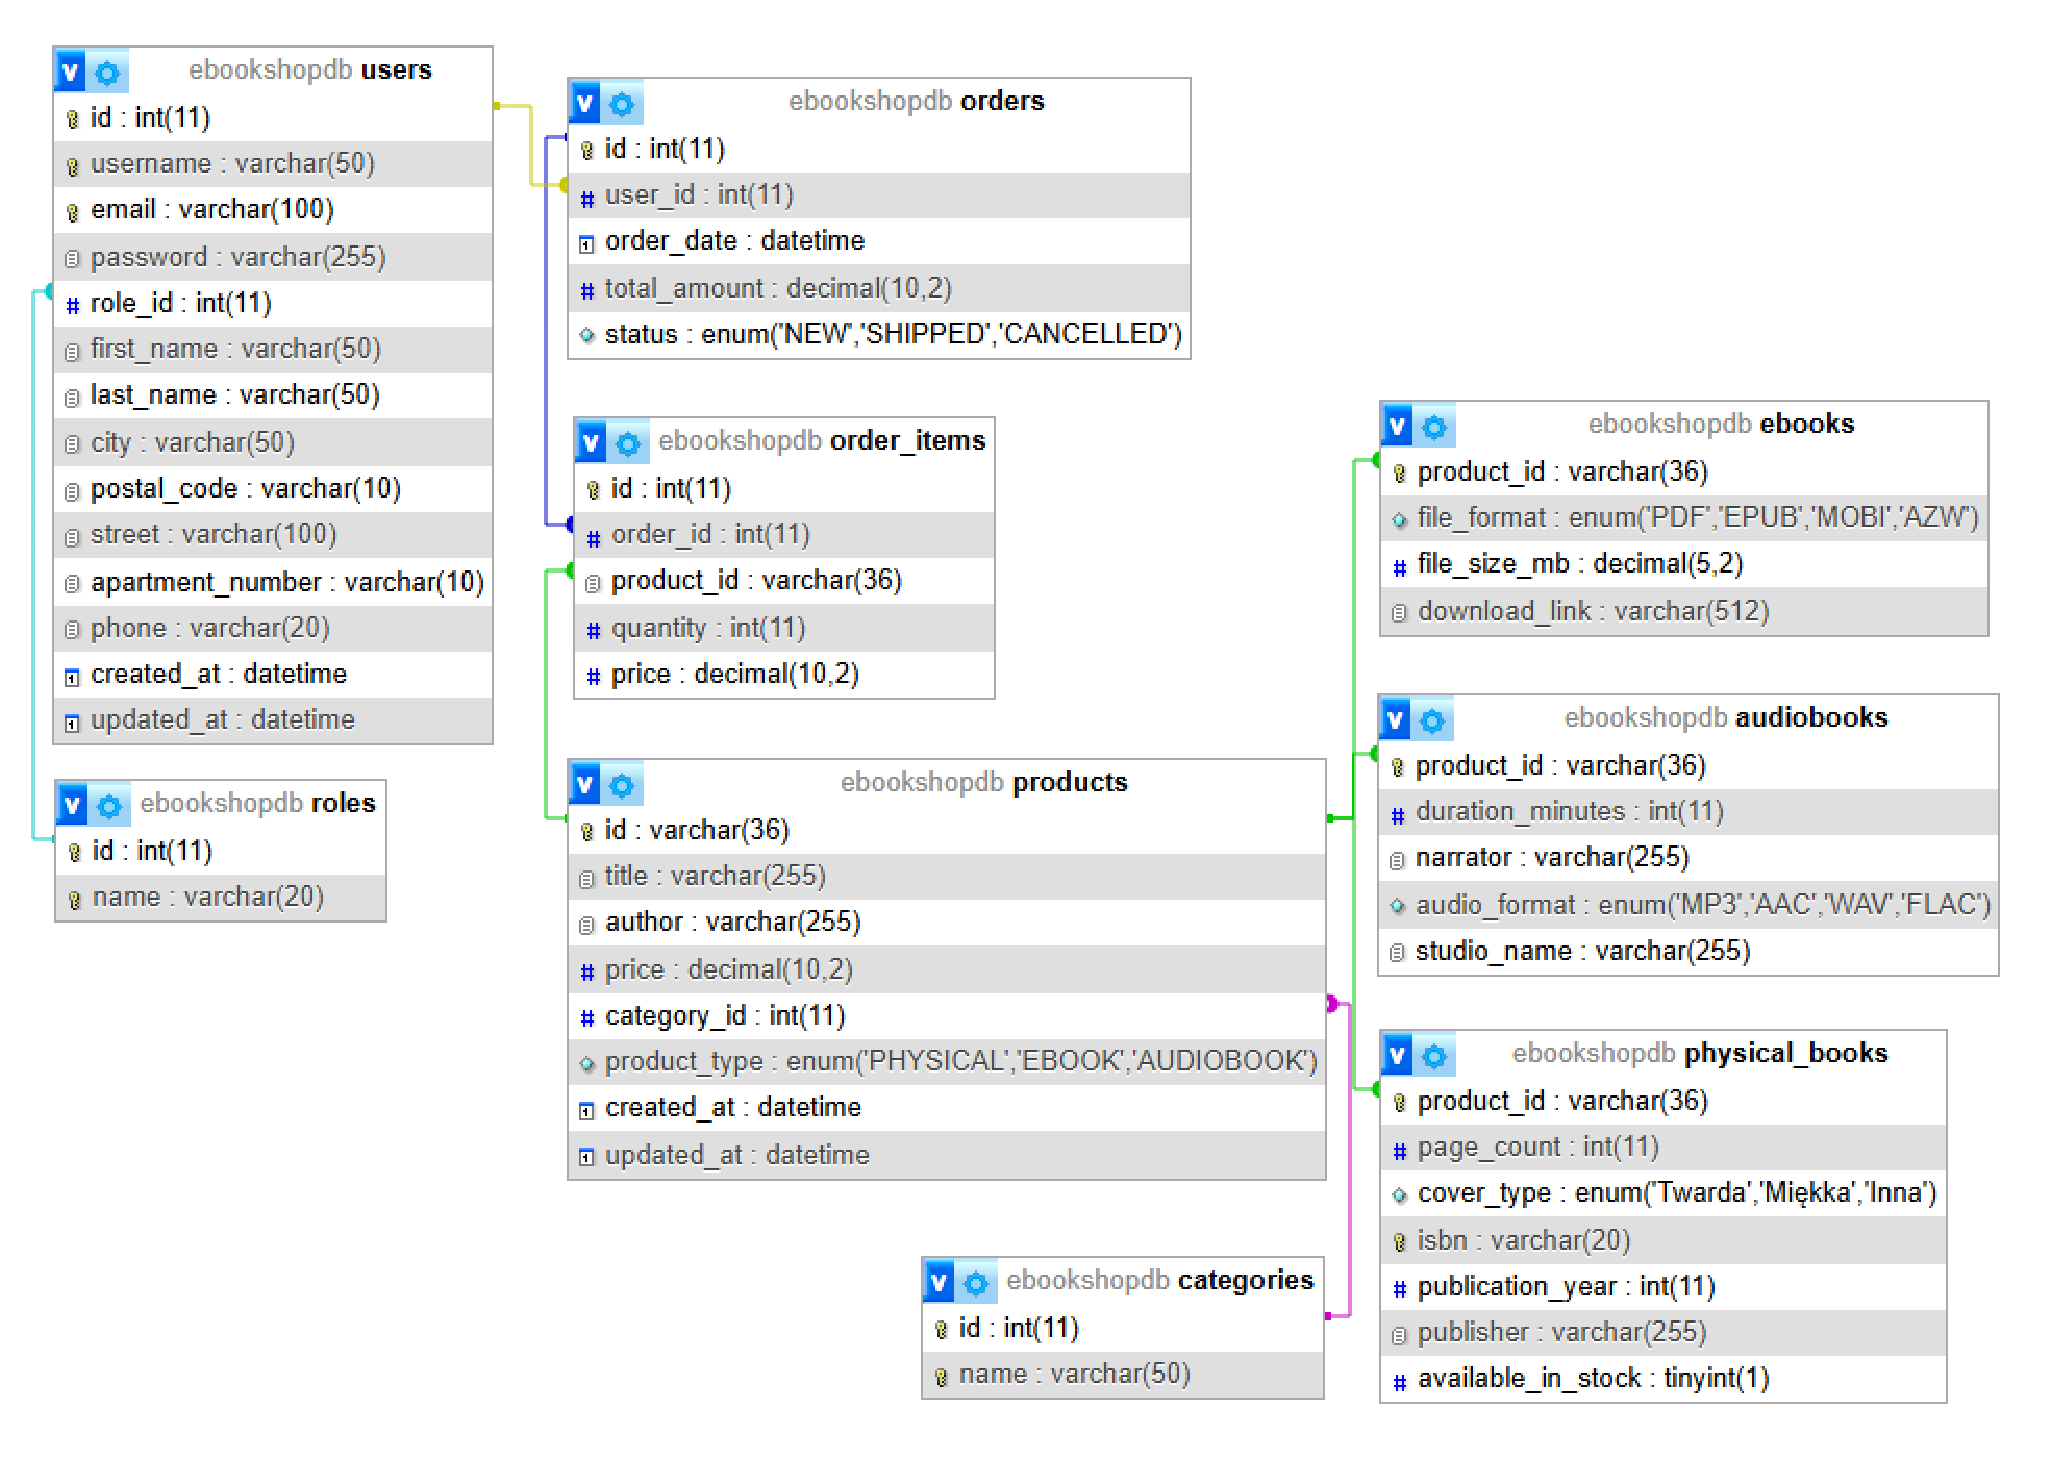
\includegraphics[width=\linewidth]{figures/fig_0004.eps}\\
    \caption{Diagram ERD bazy danych.\label{fig4}}
\end{figure}

% ------------------------------------------------------------------------

\section{Graficzny interfejs użytkownika}

% ------------------------------------------------------------------------

\subsection{Struktura GUI}

Graficzny interfejs użytkownika został stworzony w taki sposób, aby był przejrzysty, prosty w obsłudze, a także estetyczny wizualnie.
Do tworzenia GUI wykorzystana została biblioteka SWING, a do samego projektowania, rozszerzenie \texttt{SWING UI DESIGNER}.

Wszystkie elementy interfejsu graficznego przechowywane są w pakiecie \texttt{GUI}, podzielone są one na okna dostępne dla klientów oraz gości, a także okna administratora, dostępne 
w zależności od tego na konto, z jaką rolą, zaloguje się użytkownik. Struktura GUI zaprezentowana została na diagramie na \figurename~\ref{fig5}. Diagram utworzony został przy użyciu \url{https://www.drawio.com/}.
\begin{figure}[H]
    \centering
    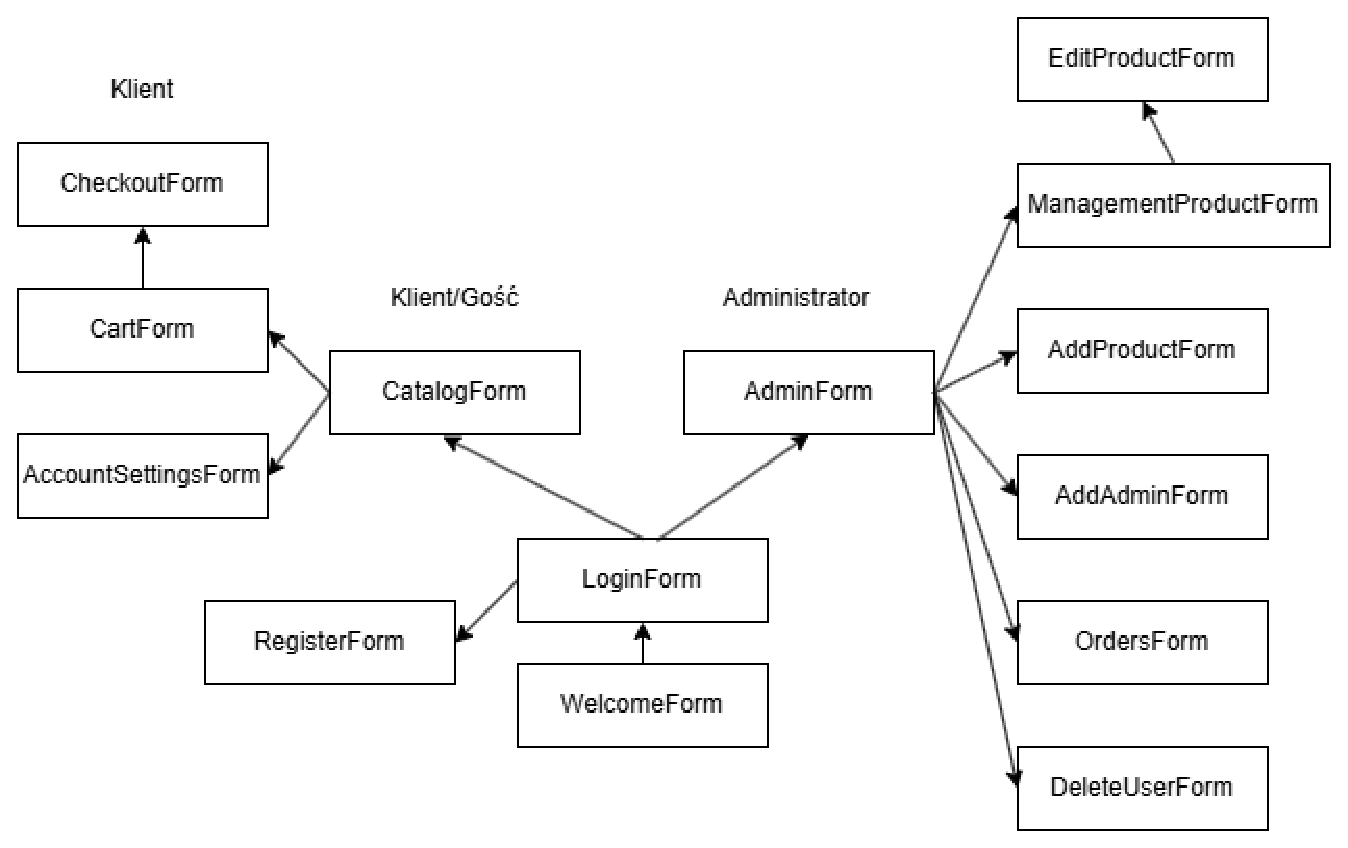
\includegraphics[width=\linewidth]{figures/fig_0005.eps}\\
    \caption{Diagram kolejnych okien aplikacji.\label{fig5}}
\end{figure}

% ------------------------------------------------------------------------

\subsection{Katalogi}

W sklepie internetowym często występują katalogi, takie jak np. katalog produktów i katalog zamówień. Jest to bardzo ważny element aplikacji, zatem konieczne jest aby były one czytelne oraz proste w korzystaniu z nich.

W projekcie wykorzystano metodę tworzenia katalogów, za pomocą dodawania do \texttt{JScrollPane} coraz to kolejnych paneli, zawierających dane na temat produktu (w przypadku katalogu produktów), a także przyciski funkcyjne
do np. dodawania przedmiotów do koszyka lub usuwania użytkowników (w przypadku panelu do usuwania użytkowników przez administratora). Wewnętrzną klasę paneli produktów prezentuje \listingname~\ref{panel}.
\lstinputlisting[caption= Klasa paneli z produktami, label=panel, style = javaStyle]{src/panel.java}

% ------------------------------------------------------------------------

\subsection{Sortowanie}

W tym przypadku katalogu produktów istotna jest również możliwość sortowania i filtorwania listy produktów. W tym celu wykorzystane zostały standardowe pakiety i klasy Javy takie jak np. \texttt{Collectors}.
Metoda \texttt{filterProducts} wykorzystuje strumień \texttt{stream} do filtrowania produktów na podstawie wybranego typu i kategorii, a następnie zbiera wyniki z powrotem do listy za pomocą \listingname~\ref{sort}.
Sortowanie natomiast odbywa się za pomocą metody \texttt{sort}, wywoływanej dla \texttt{mutableList}.\figurename~\ref{fig6} przedstawia implementację tych funkcjonalności.
\lstinputlisting[caption= Metody filtorwania oraz sortowania, label=sort, style = javaStyle]{src/sort.java}